\documentclass[12pt]{article}

% Packages
\usepackage[margin=1in]{geometry}
\usepackage{amsmath, amsthm, amssymb, physics, graphicx}

% Problem Box
\setlength{\fboxsep}{4pt}
\newsavebox{\savefullbox}
\newenvironment{fullbox}{\begin{lrbox}{\savefullbox}\begin{minipage}{\dimexpr\textwidth-2\fboxsep\relax}}{\end{minipage}\end{lrbox}\begin{center}\framebox[\textwidth]{\usebox{\savefullbox}}\end{center}}
\newenvironment{pbox}[1][]{\begin{fullbox}\ifx#1\empty\else\paragraph{#1}\fi}{\end{fullbox}}

% Options
\allowdisplaybreaks
\addtolength{\jot}{1em}
\theoremstyle{definition}

% Default Commands
\newtheorem{proposition}{Proposition}
\newtheorem{lemma}{Lemma}
\newcommand{\ds}{\displaystyle}
\newcommand{\isp}[1]{\quad\text{#1}\quad}
\newcommand{\N}{\mathbb{N}}
\newcommand{\Z}{\mathbb{Z}}
\newcommand{\Q}{\mathbb{Q}}
\newcommand{\R}{\mathbb{R}}
\newcommand{\C}{\mathbb{C}}
\newcommand{\eps}{\varepsilon}
\renewcommand{\phi}{\varphi}
\renewcommand{\emptyset}{\varnothing}

% Extra Commands


% Document Info
\title{\vspace{-0.5in}Assignment 5\\
    \large GEOG 191
}
\author{Harry Coleman}
\date{February 8, 2021}

% Begin Document
\begin{document}
\maketitle


\begin{pbox}[1]
    A company supplies goods to the three customers, each requiring 30 units. The company has two warehouses. Warehouse 1 has 40 units available and warehouse 2 has $30$ units available. The cost to ship 1 unit from warehouses to customers is given below. What is the least cost allocation of goods to customers?
    \begin{center}
        \begin{tabular}{|l|c|c|c|}
            \hline
                        & Customer 1 & Customer 2 & Customer 3 \\ \hline
            Warehouse 1 & \$15       & \$35       & \$25       \\ \hline
            Warehouse 2 & \$10       & \$50       & \$40       \\ \hline
        \end{tabular}
    \end{center}
\end{pbox}

\begin{pbox}[(a)]
    Structure this problem as a linear program.
\end{pbox}

Let $x_{ij}$ denote the number of units to be shipped from warehouse $i$ to customer $j$. Similarly, let $c_{ij}$ be the cost to ship 1 unit from warehouse $i$ to customer $j$, i.e.,
\[
    c = \mqty[15 & 35 & 25 \\ 10 & 50 & 40].
\]
Each warehouse can ship at most 40 total units and each customer requires at least 30 total units. Then we have the integer linear program
\[\begin{array}{ll}
    \textbf{Minimize} & Z = \ds\sum_{i=1}^2 \sum_{j=1}^3 c_{ij}x_{ij}, \\
    \textbf{Subject to} & \ds\sum_{j=1}^3 x_{ij} \leq 40, \quad i = 1, 2, \\
        & \ds\sum_{i=1}^2 x_{ij} \geq 30, \quad j = 1, 2, 3, \\
        & x_{ij} \geq 0, x_{ij} \in \Z \quad i = 1, 2, \quad j = 1, 2, 3.
\end{array}\]

\newpage
\begin{pbox}[(b)]
    Solve the problem using the simplex method (tableau)
\end{pbox}

We have a slack variable for each supply constraint, and we have an excess and artificial variable for each demand constraint. Since we want to minimize $Z$, we take $-Z$ for the simplex method. Explicitly, we obtain the following standard augmented form. 
\[\begin{array}{ll}
    \textbf{Maximize}       & -Z = -x_{11} -x_{12} -x_{13} -x_{21} -x_{22} -x_{31} -Ma_1 -Ma_2 -Ma_3, \\
    \textbf{Subject to}     & x_{11} + x_{12} + x_{13} + s_{1} = 40, \\
                            & x_{21} + x_{22} + x_{23} + s_{1} = 40, \\
                            & x_{11} + x_{21} - e_{1} + a_1  = 30, \\
                            & x_{12} + x_{22} - e_{2} + a_2  = 30, \\
                            & x_{13} + x_{23} - e_{3} + a_3  = 30, \\
                            & x_{11}, x_{12}, x_{13}, x_{21}, x_{22}, x_{31}, s_1, s_2, e_1, e_2, e_3, a_1, a_2, a_3 \geq 0.
\end{array}\]

I implemented the standard augmented form of the problem for the simplex method in Xpress, i.e., with the above variables and equality constraints.

\noindent
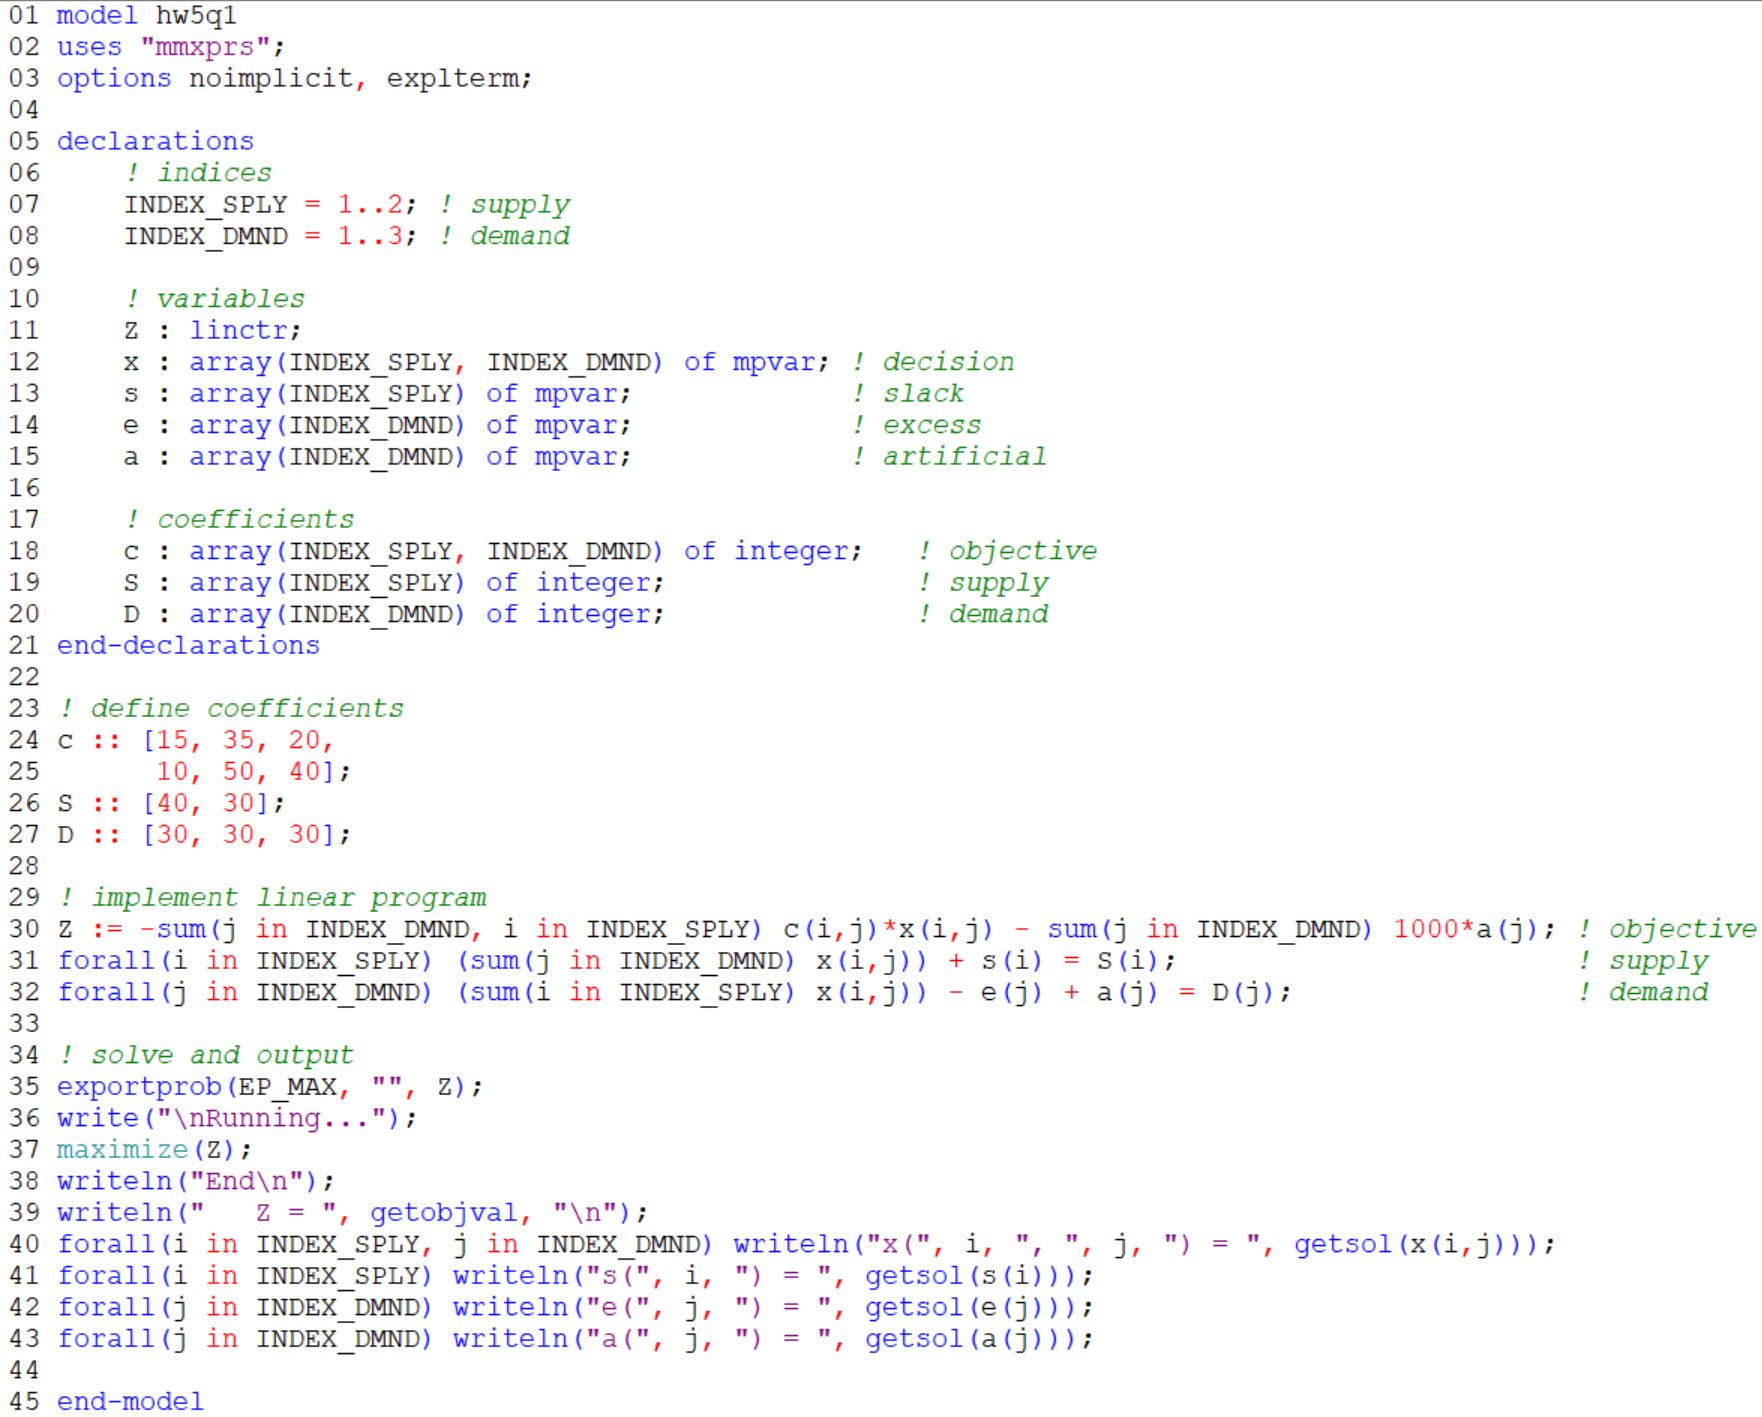
\includegraphics[width=\textwidth]{code1a.png}

\newpage
This model ran for 5 iterations of the simplex method and produced the following optimal solution.
\begin{verbatim}
           Z = -21250
    
        x(1, 1) = 0
        x(1, 2) = 10
        x(1, 3) = 30
        x(2, 1) = 30
        x(2, 2) = 0
        x(2, 3) = 0
        s(1) = 0
        s(2) = 0
        e(1) = 0
        e(2) = 0
        e(3) = 0
        a(1) = 0
        a(2) = 20
        a(3) = 0
\end{verbatim}
Since the simplex method terminated with a nonzero artificial variable, then we can conclude that the original linear program is infeasible. This is clear in the original problem, as the total demand is 90 units, but the total supply is only 70 units.






\newpage
\begin{pbox}[3]
    Coach Macedo of the UCSB Swim team is putting together a medley relay of swimmers for an upcoming meet. Each swimmer is assigned a 100 m stroke (free, breast, fly, and back), and can only swim one leg of the relay. Coach Macedo seeks the fastest relay, with best individual times this season indicated in the below table. What is the best configuration of the relay team?
    \begin{center}
        \begin{tabular}{|l|l|l|l|l|}
        \hline
                & Free & Breast & Fly & Back \\ \hline
        Natalie & 54   & 54     & 51  & 53   \\ \hline
        Brynn   & 51   & 57     & 52  & 52   \\ \hline
        Angie   & 50   & 53     & 54  & 56   \\ \hline
        Holly   & 56   & 54     & 55  & 53   \\ \hline
        \end{tabular}
    \end{center}
\end{pbox}

\begin{pbox}[(a)]
    Structure this problem as a linear program.
\end{pbox}

Let $I$ and $J$ be indexing sets for the players and strokes, respectively, i.e.,
\begin{align*}
    I &= \{\text{Natalie}, \text{Brynn}, \text{Angie}, \text{Holly}\}, \\
    J &= \{\text{Free}, \text{Breast}, \text{Fly}, \text{Back}\}.
\end{align*}
Let $x_{ij}$ be the binary decision to have swimmer $i$ swim stroke $j$. Similarly, let $c_{ij}$ be the time swimmer $i$ takes to swim 100 m with stroke $j$, i.e.,
\[
    c = \mqty[54 & 54 & 51 & 53 \\ 51 & 57 & 52 & 52 \\ 50 & 53 & 54 & 56 \\ 56 & 54 & 55 & 53].
\]
Exactly one swimmer must swim each stroke, and each player can swim at most one stroke (It also happens that each player swims exactly one stroke, but this would not necessarily be the case if there were more swimmers). So we obtain the following binary linear program
\[\begin{array}{ll}
    \textbf{Minimize} & Z = \ds\sum_{i\in I} \sum_{j\in J} c_{ij}x_{ij}, \\
    \textbf{Subject to} & \ds\sum_{j\in J} x_{ij} \leq 1, \quad i \in I \\
        & \ds\sum_{i\in I} x_{ij} = 1, \quad j \in J, \\
        & x_{ij} \in \{0, 1\} \quad i \in I, j \in J.
\end{array}\]

\newpage
\begin{pbox}[(b)]
    Solve the problem using the simplex method (tableau)
\end{pbox}

To put this problem into standard augmented form for the simplex method, we would add a slack variable for each swimmer constraint and an artificial variable for each stroke constraint. I implemented the linear program from (a) in Xpress.

\noindent
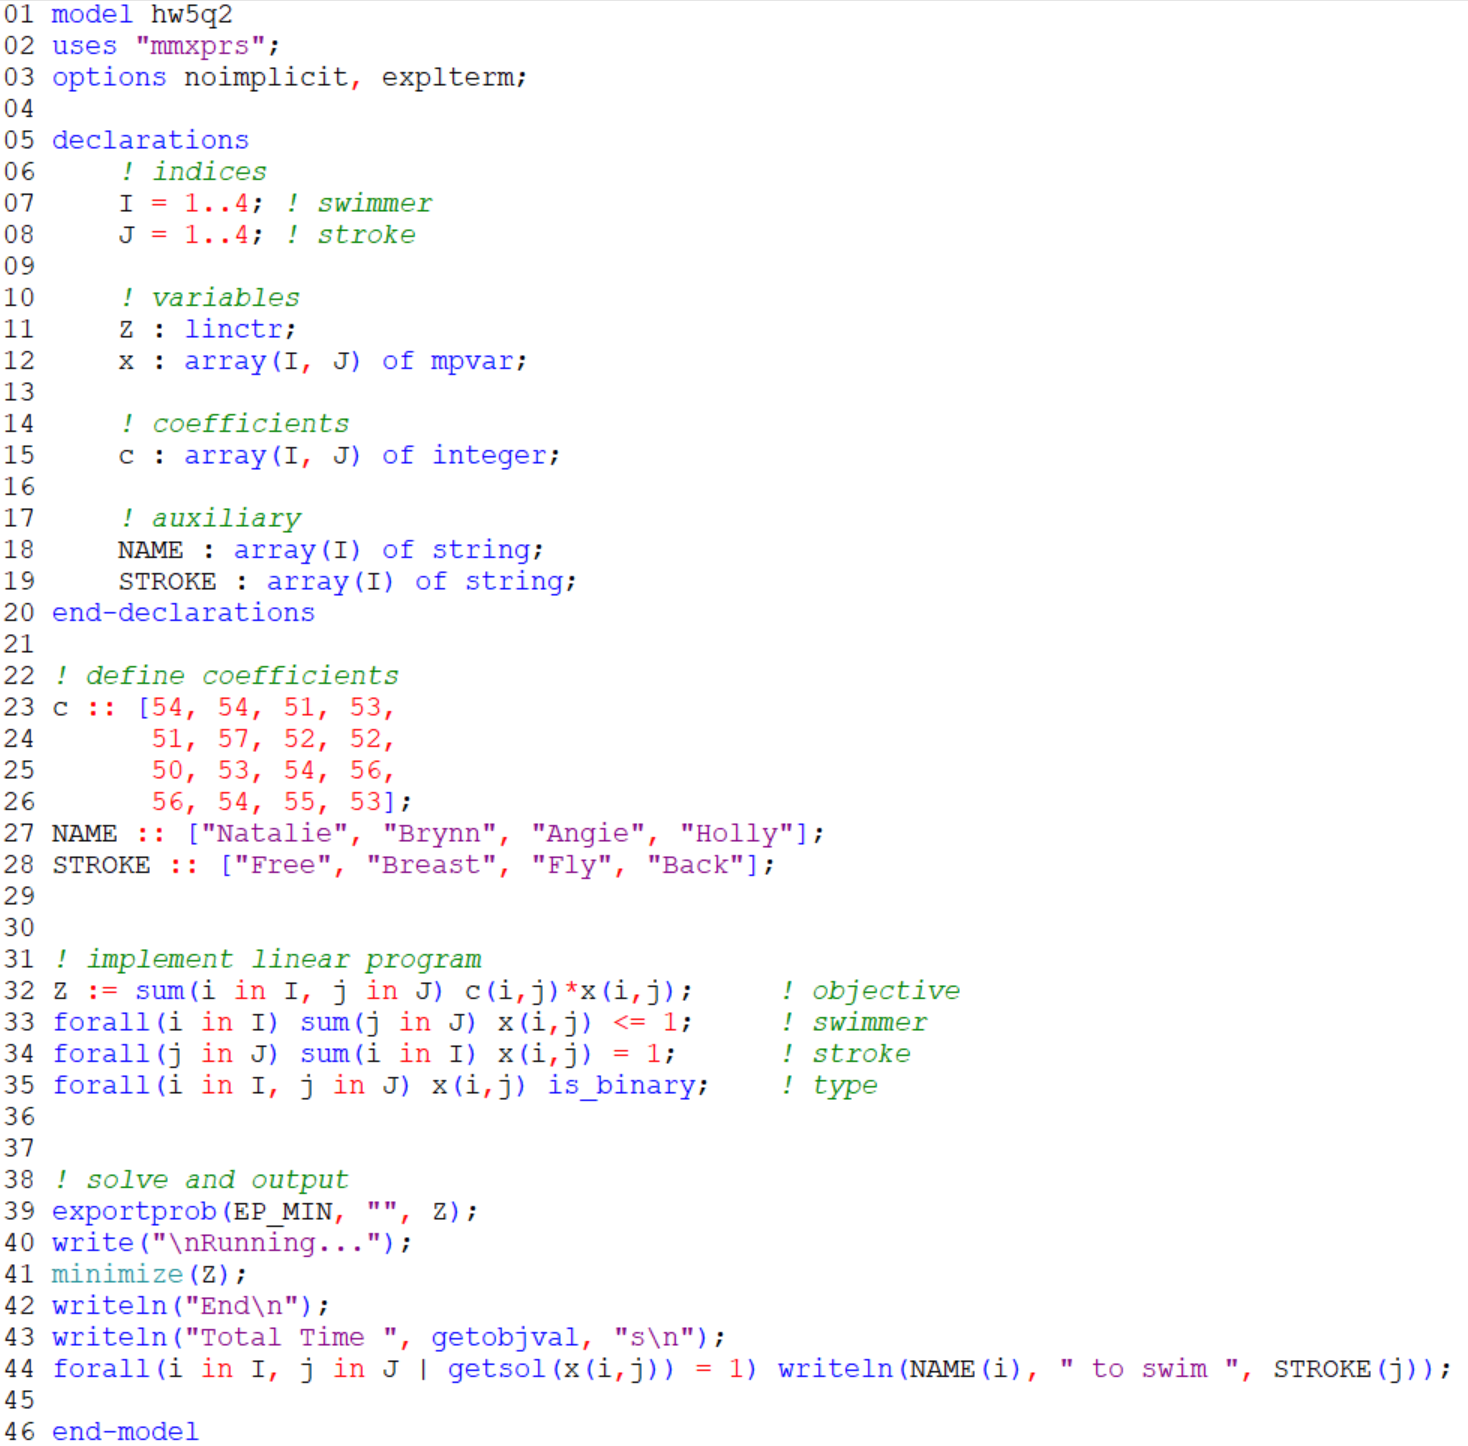
\includegraphics[width=\textwidth]{code2.png}
This model produces the following optimal solution.
\begin{verbatim}
    Total Time 207s

    Natalie to swim Fly
    Brynn to swim Back
    Angie to swim Free
    Holly to swim Breast
\end{verbatim}

\end{document}